% !TeX spellcheck = en_GB
% !TeX spellcheck = en_US 
\chapter{Theoretical Background}

In this chapter we will present all the theoretical background necessary for the development of this project, from the creation and behaviour of the Helium and Neon droplets to the theory of the plasma formation and the coulomb explosion processes. In order to guide the reader in an organized way, the sections are organized in the same order the experiment is performed.


\section{Helium Nanodroplets}

The combination of cryogenic matrix isolation, discovered in 1954 \cite{whittle_matrix_1954}, and the now well-defined properties of helium (He), especially its superfluity phase discovered in 1937 by \textit{Kapitza et al} \cite{kapitza_viscosity_1938}, gives as a consequence, an excellent molecular matrix like the helium nanodroplets.
Helium has unique properties that make it a perfect source for the nanophysics experiments. For example, it has any optical transitions in the entire infrared and visible regime. In addition, helium clusters are able to pick up atoms and molecules that form different complexes of the species embedded in the interior or the surfaces of the droplet, acting as an ideal matrix for spectroscopy of atoms and molecules. \cite{stienkemeier_spectroscopy_2006}\cite{toennies_superfluid_2004}.

The size of a Helium cluster can be up to $10^{8}$ atoms, and reach the ultra-cold temperature regime (close to 0.37 K \cite{toennies_spectroscopy_1998})\cite{enss_low-temperature_2005}.
Two main advantages of this cooling properties arise. First, dopants in the helium nanodroplet are set to their absolute vibronic ground states, avoiding other possible spectra and establishing the cluster in a specific state. Second, the fast cooling helps in the formation of isomers that are difficult or impossible to generate with other methods \cite{nauta_nonequilibrium_1999}. Third, because the superfluid phase of the helium \cite{grebenev_superfluidity_1998}, the bond between dopants and helium is weak. Therefore, in contrast to spectroscopy in other matrices with higher temperatures, the optical transitions of many dopants are barely influenced by the helium matrix \cite{toennies_superfluid_2004}. 
The theory of He super fluidity will not be part of this section, this information is well documented in other sources, and here we are based on ref.\cite{enss_low-temperature_2005} where all theory is well presented to the reader. In the next section we will dedicate a bigger effort to explain the theoretical and technical background of the helium nanodroplets creation as well as the physical and technical process to dope it. 

\subsection{General Properties of Helium}


At room temperature, helium is a light inert gas. It is odorless, colorless, tasteless, and after hydrogen, the second most abundant element in the universe.  \cite{enss_low-temperature_2005}. It has a simple 2 atoms structure, exhibiting numerous exotic phenomena whose theoretical descriptions are rather complex in many cases, i.e it characteristics of a quantum fluid. From helium exist two stable isotopes $^{3}He$ and $^{4}He$.  $^{4}He$ has two electrons, two protons and two neutrons, no nuclear spin and no total spin, pertaining to the bosonic family, while $^{3}He$ with only one neutron has a spin of $I = 1/2$ and belongs to the fermions \cite{atkins_liquid_2014}.

The bosonic state $_{4}He$ is especially of interest, at  temperature T$\leqslant$2.8K and under normal pressure has a phase transition from "normal liquid" $He-I$ to super liquid $He-II$ \cite{swenson_liquid-solid_1950}, in which the helium can be described by a Bose-Einstein condensation. Even the fermionic $^{3}He$ exhibits this phase transition at T$\leqslant 0.03K$ \cite{halperin_properties_1978}.

The superfluidity of helium two (He-II), at temperatures close to absolute zero, brings with it some unique features. The essential Properties for this include an almost disappearing viscosity in the superfluid phase, weak interaction, very efficient cooling, and the transparency for electromagnetic radiation up to wavelengths in vacuum ultraviolet (VUV) Spectral range \cite{enss_low-temperature_2005}. Helium has therefore in the complete visible spectrum no transitions from the ground state. Through the noble gas configuration, helium has a spherically symmetrical electron distribution \cite{lewis_Helium_2014}, it can hardly be polarized and is the least reactive of all the elements.

\begin{figure}[h!]
\centering
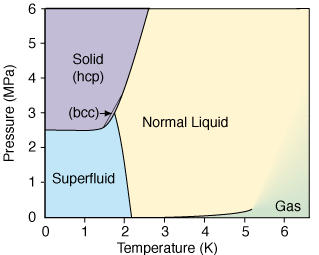
\includegraphics[width=8 cm]{../Images/He_temp_phases.png}
\caption[Helium phase diagram]{$^{4}He$ Phase transition at Ultra cold temperatures. $^{4}He$ is the more common isotope of helium. It remains liquid at zero temperature if the pressure is below $2.5 MPa$. The liquid has a phase transition to a superfluid phase, also known as Helium-II, at the temperature of $2.17 K$ (at vapor pressure). Taken from \cite{noauthor_Helium_nodate}}

\end{figure}


\subsection{Helium Droplets}

The production of Helium droplets had to overcome first one principal problem, its condensation. At the end  of the 19th century, many noble gases were liquefied for the first time by applying pressure at room temperature. However, for helium and hydrogen, this method was not successful. In 1922 Kamerlingh Onnes reached temperatures below $1$ K by reducing the vapor pressure above liquid helium to about $2*10^{-5}$ bar with a series of pumps \cite{van_delft_discovery_2010}. The Joule–Thomson effect \cite{weinberger_discovery_2013} was the responsible for Onnes experiment to reach this low temperature. The basic idea is that under suitable conditions an expanding gas performs work against its internal forces, for example, when a gas is expanded through a small nozzle thermally isolated from its surroundings. The expansion under these conditions takes place at constant enthalpy, since the expansion nozzle performs none work. It follows the next relation.

\begin{equation}
W= H_{1}-H_{2} = (U_{1}+p_{1}V_{1})-(U_{2}+p_{2}V_{2})
\end{equation}


Where H is the enthalpy before and after, $U=\dfrac{3}{2}Nk_{b}T$ is the internal energy, and follows the  ideal gases law $pV=Nk_{b}T$ \cite{enss_low-temperature_2005}. Under Joule–Thomson effect conditions, $W=0$ so $H_{1}=H_{2}$, this expansion leads to a cooling or a warming,  bank on the conditions it becomes supersaturated. As a result, condensation takes place and a beam of clusters is formed.

Helium nanodroplets are typically produced by a continuous or pulsed adiabatic expansion of pre cooled gas through a small aperture from a reservoir into a vacuum \cite{stienkemeier_spectroscopy_2006}. In this process a droplet jet is formed, and its characteristics (blasting speeds and size distribution) can be changed due to the manipulation of the setup. For example, pressure differential between the reservoir and the vacuum chamber (usually in the range of a few to $10$ MPa), the nozzle temperature (from a few K to $T \leqslant 40$ K) or the nozzle size (with pinholes of diameter rounding $5-20 \mu$m).



\begin{figure}[h!]
\centering
	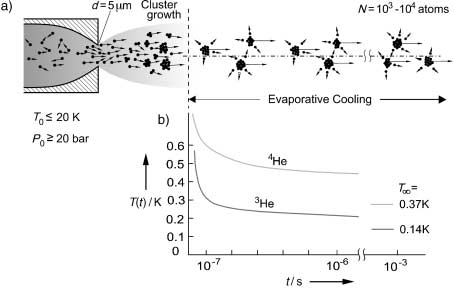
\includegraphics[width=0.6\textwidth]{../Images/jet_scketch.png}
	\caption[Scheme for a nozzle expansion]{ a) Schematic representation of the processes leading to the formation and subsequent cooling of Helium droplets in a gas expansion. b) Calculated dependence of the droplet temperature on time for $^{4}$He and $^{3}$He droplets after they have left the cluster, taken from \cite{toennies_superfluid_2004}	}
	\label{img:jet}	
\end{figure}

\begin{figure}[h!]
\centering
	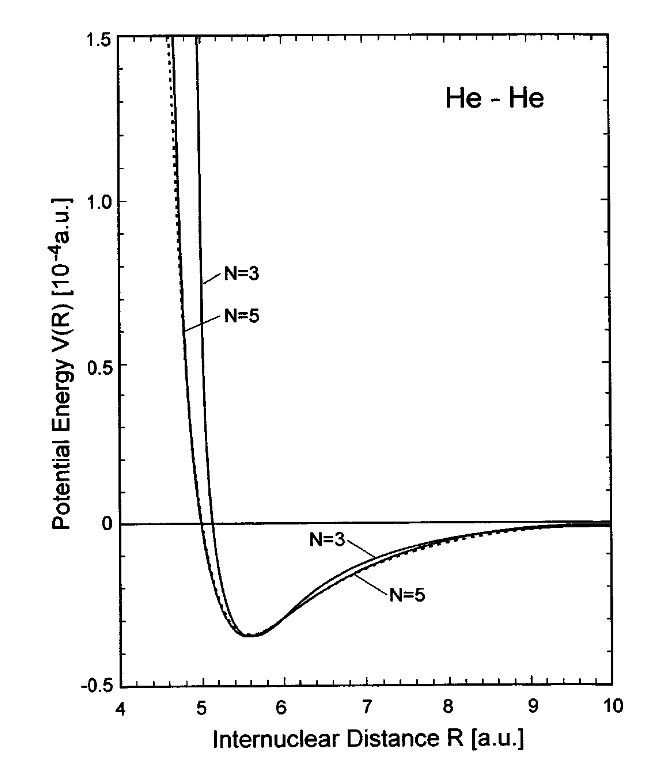
\includegraphics[width=0.5\textwidth]{../Images/waanderwaal_hehe.PNG}
	\caption[Waan der Wall He-He potential]{ Van der Waals potential for He-He interaction. Taken from \cite{blanco_quantum_2010}}
	\label{img:WanderHe}
\end{figure}

When the Helium expands after the nozzle, its potential energy alters to kinetic energy  in a supersonic flow field. After the expansion into the vacuum, the gas becomes supersaturated and condensation occurs, creating the beam cluster. These clusters are made of atoms or molecules, held together by Van der Waals forces, in this case He-He interaction, that share the same kinetic vector. This means that, the two particles travel as close and parallel to each other so  bonding is possible as shown in Fig \ref{img:WanderHe}. From the reference frame of the cluster, each of its molecules is close to zero movements, in Helium this enhance the conditions to be liquid and in consequence, superfluidity is achieved \cite{hagena_cluster_1972}.
 

Depending on the buffer gas used, the mechanisms for cluster formation in the supersonic expansion range as a condensation either from the gas phase or the liquid phase. In case the expansion is isentropic (adiabatic and reversible), the expansion is represented by a vertical line in this diagram. Clusters formed by condensation from the gas phase occur when the expansion crosses into the two-phase region on the right-hand side of the critical point. Clusters formed by fragmentation of the liquid phase occur when the expansion crosses into the two-phase region on the left hand side of the critical point. The diagram is an example of three gases, He, Ar and H$_{2}$ at different pressures ($p'=P/P_{critical},$)\cite{knuth_average_1999}. The curves represent the regions where the supersonic expansion is possible and the temperatures (in Fig dimensionless) that each gas should have in order to achieve clustering and cooling \cite{knuth_average_1999}.

\begin{figure}[h!]
	\centering
	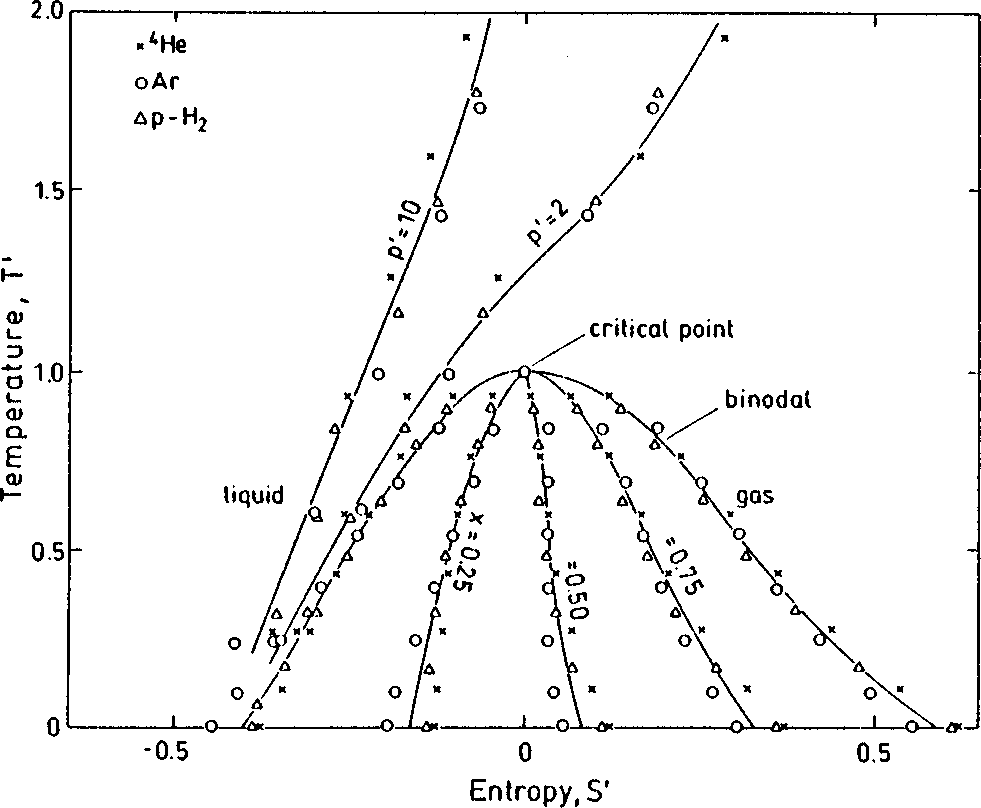
\includegraphics[width= 8 cm]{../Images/dimensiones isentropic diagram.png}
	\caption[helium isentropic diagram]{Dimensionless phase diagram for He, H2 and Ar. Where T is dimensionless $T'=(T -T_{tp})/(T_{cr}-T_{tp})$, same as entropy $S'=(S-S_{cr})/\Delta S_{tp}$ and $x$ is the fraction of the fluid in the gaseous phase, where the subscripts $cr$ and $tp$ refer to the critical point and triple point respectively, and $\Delta S$ is the entropy change for vaporization. The curves are drawn as guides to the eye, not exact measurements, taken from \cite{knuth_average_1999}.}
	\label{img:tsHe} 
\end{figure}
  

There is no mathematical approach of the physics behind this supersonic expansion but usually, Raleigh scattering measurements in combination with an empirical scaling law \cite{hagena_cluster_1972} are used to estimate the mean cluster size, assuming a certain degree of control over the cluster size distribution by adjusting the nozzle width and the source pressure. The droplet size distribution during supersonic expansion in the follows a log-normal distribution of the form \cite{harms_density_1998}.

\begin{equation}
p(N) = \frac{1}{\sqrt{2\pi}N \sigma} \exp  \left[- \frac{(ln(N/N_{0})^2}{2\sigma^2} \right]
\end{equation}

Where \textit{N} is the number of atom in the cluster, $\sigma$ is the distribution width and \textit{$N_{0}$} is the most likely numbers of atoms. Following it give a mean value.

\begin{align}
\bar N = \exp  \left(\mu+\frac{\sigma^2}{2} \right)
\end{align}

With a half width maxima of \cite{harms_density_1998}

\begin{align}
\sigma N_{\frac{1}{2}} = \exp \left( \mu - \sigma ^2 + \sigma \sqrt{2 ln(2)} \right) - \exp \left(  \mu - \sigma ^2 - \sigma \sqrt{2 ln(2)}  \right)
\end{align}

\begin{figure}[h!]
\centering
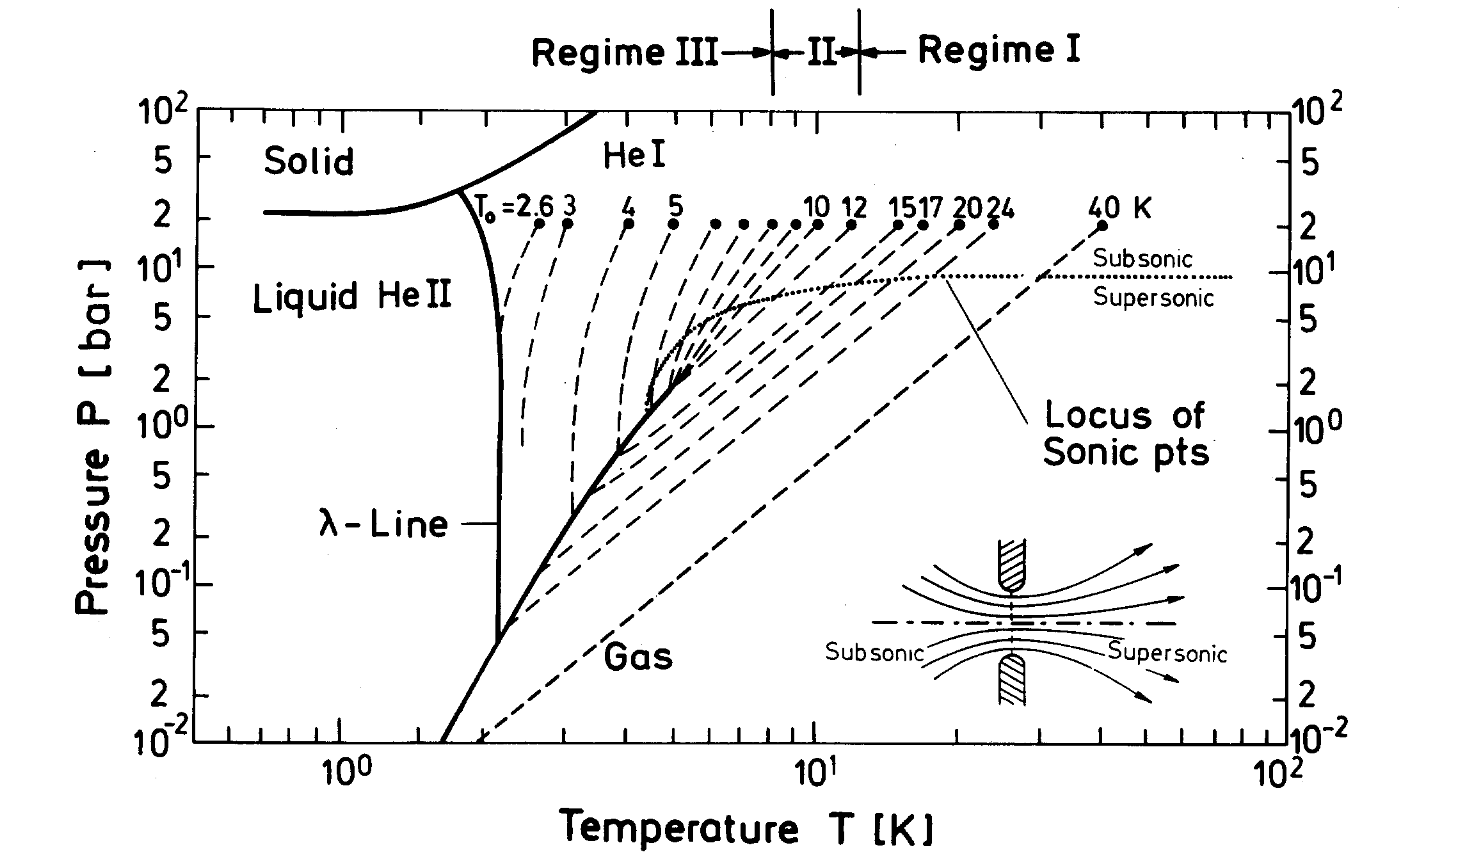
\includegraphics[width= 10cm]{../Images/expansion_regimes.PNG}
\caption[Phase diagram for Expansion regimens]{Expansion regimes. $^{4}$He Pressure-Temperature phase diagram for Nozzle beam expansions starting at a backing pressure  of 20 bar and $a$ temperature. As discussed, qualitatively different behaviors are shown for the regime I-II and II where starting in the gas phase,  near the phase transition respectively. Taken from \cite{buchenau_mass_1990}. }
\label{fig:ExpRegim}
\end{figure}

As show in Figure \ref{fig:ExpRegim}, the initial gas conditions (pressure, temperature and nozzle size) in the free expansion phase will determine the characteristics of the final helium beam. From here, three main regimes can be define.

Regime I or sub-critical expansion, begins in the gas phase and leads to droplet formation via condensation. This is the case of most expansions since the pressure is located below the critical pressure $P_{c}$.
Regime II, also called as critical expansion, is a long-winded regime that includes all trajectories which are near the critical point, leading to random expansion and difficult control of the beam due the large fluctuations in density.
Regime III, the super-critical expansion, starts at low temperatures where the helium stops behaving as an ideal gas, expecting flashing or cavitation  breaking up the liquid drops jet. \cite{buchenau_mass_1990}

super-critical and sub-critical regimes have been studied  in the last several years and  are clearly identified in the resulting size distributions. Figure \ref{img:dropletSize} shows that super-critical expansion forms large droplets (usually between $20-100$ nm diameter) while a sub-critical expansion is suited to generate small droplets (around $5-10$ nm).  A simple relation that can be done to calculate the size or number of atoms in a Custer is using. 

\begin{equation}
r=N_{1/3} * \rho A
\end{equation}

Where $r$ is the radius of the beam, and $\rho$ its density, in this case, for helium $\rho =0.0022$ A  \cite{stringari_systematics_1987}, but this approximation is not exact due the variation in He density at this temperature. As expected in both regimens, for creating larger helium nano droplets, higher He pressure and lower nozzle temperature are used. For our experiment a $5 \mu$m nozzle was used at temperatures oscillating between $11-20 K$, and backing pressures of $30, 45 $ and $ 50$ bar.

\begin{figure}[h!]
\centering
\label{img:dropletSize}
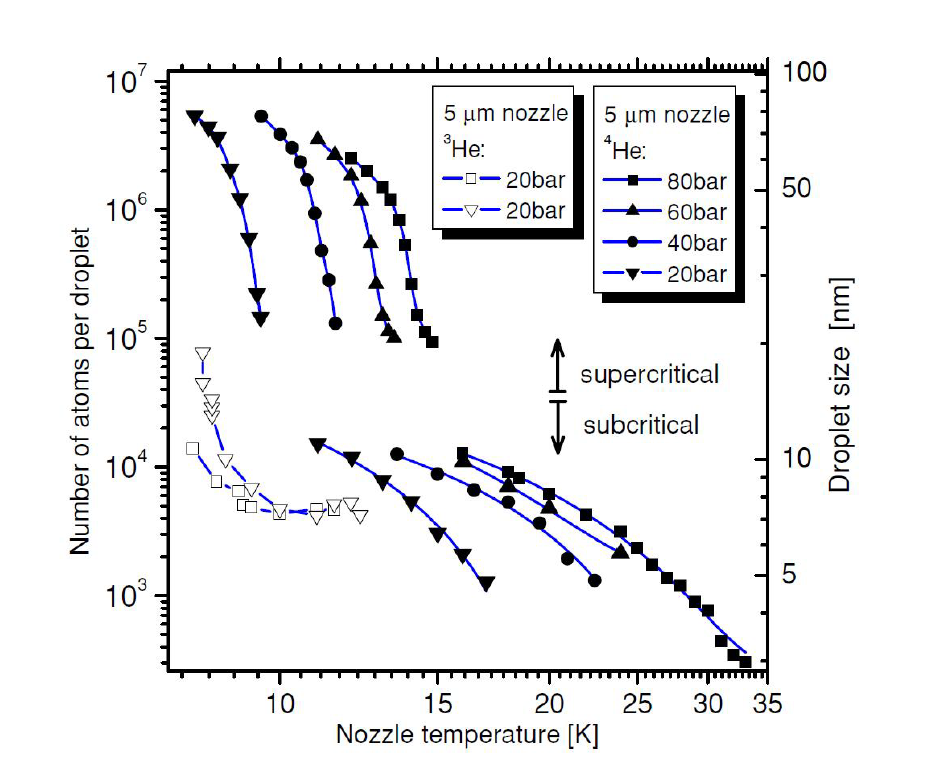
\includegraphics[scale=0.4]{../Images/sizes_regimen.PNG}
\caption[Expansion droplets Regimens]{Sizes of the $^{4}$He droplets  as a function of nozzle temperature T and  pressures, based on \cite{toennies_spectroscopy_1998}, using a $5 \mu $m nozzle. The sub and super critical regimes are clearly differentiated. Taken from \cite{stienkemeier_spectroscopy_2006}}
\end{figure}

\section{Neon Clusters}

Neon (Ne) is the second lightest inert gas with atomic number 10, it has 3 stable isotopes in nature, the $^{20}$Ne with more than 90$\%$ of abundance, followed by $^{21}$Ne and  $^{22}$Ne \cite{meija_atomic_2016}. At extreme temperature, Neon is solid as shown in the graphic \ref{fig:Nephases} and its triple point is around $T_{p}=24$K \cite{young_phase_nodate}. Neon is a noble gas, it shares most of the properties already mentioned from Helium, except for its superfluidity.  It has a a quite large ionization potential for its first electron at $Ip=21.56$ eV, what makes quite suitable to use it as a matrix with strong fields lasers, because at low intensities, it will not interact with the light source, so dopants can be carried out in a non-interactive way.
  

\begin{figure}[h!]
\centering
\begin{subfigure}[l]{1\textwidth}
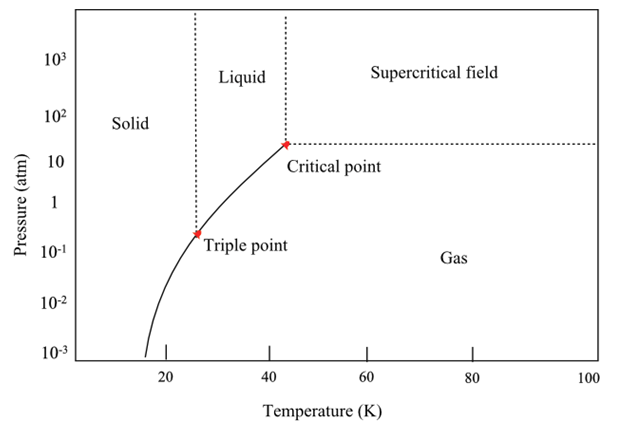
\includegraphics[width=0.45\textwidth]{../Images/Ne_temp_phases.png} \hfill
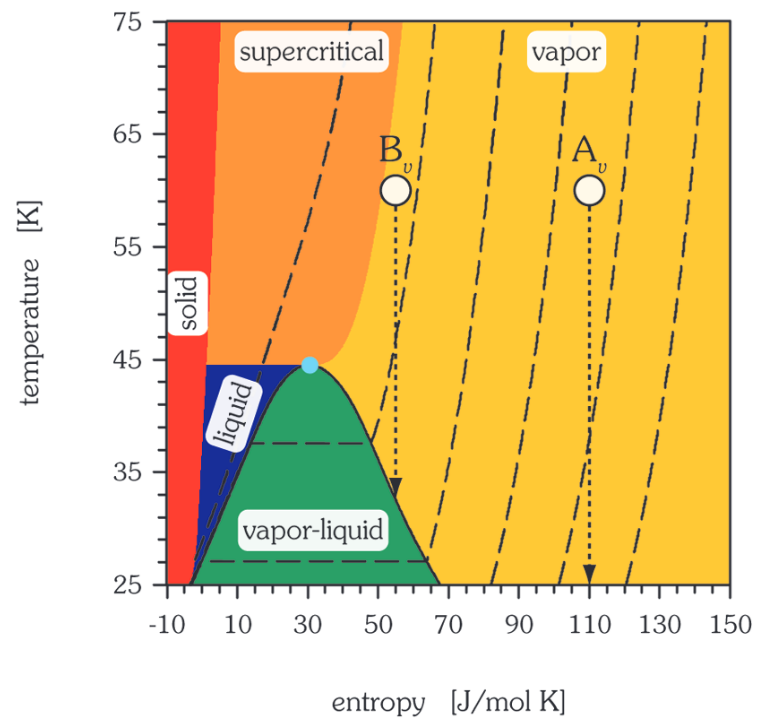
\includegraphics[width=0.4\textwidth]{../Images/T-s ne phase diagran.png}
\end{subfigure}
\caption[Neon phase-Isentropic diagrams]{On the left, Neon phase diagram. taken from \cite{young_phase_nodate}, on the right, $T-S$ phase diagram of Ne. The critical point is located at $T_{c}= 44.49$ K and a molar entropy of $S_{c}=30.76$ J/(mol K). The dashed lines represent regions. Taken from \cite{christen_supersonic_2010-1} }
\label{fig:Nephases}
\end{figure}

Ne cluster has been proved to provide an ideal medium for chemical reactions as solvation effect and heterogeneous chemistry at a microscopic level \cite{gough_infrared_1985}. With a properly regulated pick-up system the reactants are deposited in a controlled way in the cluster and it becomes a nanoreactor equivalent \cite{gaveau_reaction_2001}.

The conditions for creating Neon clusters are quite similar to the ones explained above, also well explained in the famous Hagena law \cite{hagena_cluster_1972-1}. Several studies have been realized on the characterization of Ne clusters, for example  by \textit{R. Von Pietrowski et al}   \cite{von_pietrowski_fluorescence_1997} who studied the Electronic excitations of Xe atoms and Xe$_{2}$ molecules  embedded in free Ne clusters. On contrary to helium, is important to work with neon clusters at temperatures and pressures far from its solidification point. At extreme low temperatures, small differences in pressure leads to big size changes on the clusters, the higher the pressure in the nozzle the bigger the droplets. As an example, in \textit{Pietrowski} work, it was shown that small droplets, $N=300$, where $N$ is the number of atoms in the cluster, are in a "liquid" state but for bigger droplets solidification starts to be present. In addition, the location of the dopant will be affected drastically by these sizes changes. When the droplet is in a liquid state the dopant atoms are free to move to the center contrary to denser droplets, where the dopant will stay at the surface.


The T-S representation of Helium, Fig \ref{fig:Nephases} shows the isentropic processes as simple vertical trajectories. One advantage in this color plot is the visibility of the two-phase region where condensation may take place. The dashed lines represent isobar lines at p$= 100,1000,1000,10000,$ and $100000$ Pa from left to right respectively. On one hand, supersonic expansions which originate in the vapor phase, at a very low source pressure equivalent to a comparatively large stagnation entropy $s_{0}$, will not reach this region. On the other hand, for negative entropies the solid state is always reached although for lower temperatures and a relative small entropy, the liquid state is the predominant.\cite{christen_supersonic_2010-1} 

\section{Composite Clusters}

We can define a composite cluster or doped cluster, as an atomic lump that contains one or more different atomic elements. The main interesting properties in non-doped clusters are usually set as a function of its size, but for doped clusters, the interaction between the elements creates new degrees of freedom that makes more complex its interaction. For example, the new mixture will have different structural properties due the spatial distribution of the species \cite{stienkemeier_spectroscopy_2006}. Hence, composite clusters exhibit a more diverse behaviour and offer more opportunities to study different characteristics of the material.

The difficult problem to overcome in composite cluster is how to create them. Two techniques can be used. The first one, is the co-expansion of a previous mixed gas \cite{tchaplyguine_variable_2004}. The second one is to produce first the cluster and then cross it with an atomic beam of the doping species.

For the first technique, clusters are produced by adiabatic expansion of mixtured gas through  a  narrow  conical  nozzle into vacum\cite{tchaplyguine_variable_2004}. The  cluster  formation  process  in  the coexpansion of a binary mixture is less well known beacuse it envolves several technical problems, depends on possible interactions between the elements, the condensation ranges of the bulks and even in the affinity  of the materials\cite{reinhard_introduction_2004}.

The second thechnique, used in this study is the one called pick-up process \cite{gough_infrared_1985}. The idea is simple, as a snowball on its way downhill collects or pick-up more snow, the helium cluster after being directional selected through a skimmer, passes through a doping cell full of a dopant gas at low densities ($10-2 Pa$) \cite{stienkemeier_spectroscopy_2006}. As a result, the gas atoms that are along the droplet cross sections will be captured by the beam and travel with it. The probability for Helium droplets to collect $k$ atoms or molecules via inelastic collisions depends on the length of the oven cell $l$, the cross section of the droplets $\sigma $, and the particle density inside the cell $n$. As $l$ and $\sigma $ remains constant, varying the density in the doping cell can regulate the abundance of $k$, following Poissonian statistics.

\begin{equation}
P_{k}(l,n,\sigma)=\dfrac{(ln\sigma)^{k}}{k!} e^{(-ln\sigma)}
\end{equation}

Two important properties of these relations can be deduced. First, the maxima of different cluster sizes  are equidistant, $n_{max}=\dfrac{k}{l\sigma}$ and second, the exponential function in the equation  becomes  nearly  one for  small  particle  densities \cite{bunermann_modeling_2011}.

Every pick-up process leads to an energy transfer to the droplets. As the dopant rapidly cools down, that means an energy transfer to the Helium, causes an evaporation of some He atoms to keep the temperature unchanged in the cluster. This Helium evaporation or "shrinkage", leads to a decrease in the cross section of the droplet and the probability to collect further particle. At a certain energy entry, the complete droplet evaporates if to many dopants access to it. With the average kinetic energy $E_{kin}$, and $E_{in}$ the internal.  The involved energy is composed of the following contributions \cite{bunermann_modeling_2011}.

\begin{equation}
E=\langle E_{kin}\rangle + E_{in} + E_{binding} + E_{cluster}
\end{equation}

Where

\begin{equation}
\langle E_{kin}\rangle \approx \dfrac{3}{2}k_{b}T + \dfrac{1}{2} m v^{2}
\end{equation}

Is the final kinetic energy of the droplet depending on it mass, velocity and temperature in the gas cell.


\begin{figure}[h!]

\centering
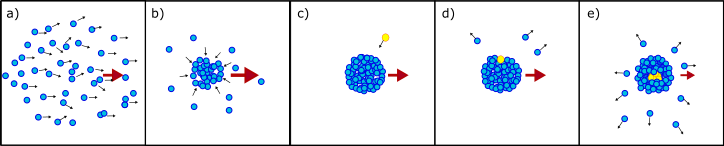
\includegraphics[width=14cm]{../Images/He_evaporation (2).png}
\caption[Helium creation, doping and evaporation sketch]{Animation of the Helium creation, doping and evaporation. From left to right, we see the Helium droplet production; after being released by the supersonic jet, the Cluster formation, the pickup process of the dopant and finally the Helium shrinking process.}
\label{fig:shrink}
\end{figure}

Several studies have focused on the $E_{binding}$ with $^{4}$He,  so the energy binding  for a broad number of materials is known. It is also important to take into account that the binding energy includes the cluster-dopant binding as well as the dopant-dopant relation.\cite{toennies_spectroscopy_1998}. The energy bounding for example of Xe-He is arround $26.9 $ meV \cite{lewerenz_successive_1995}, or He-H$_{2}$O is about $0.1$ eV \cite{lewis_Helium_2014}.

\section{Cluster-Intense Fields  Interaction}


The understanding of the interaction atom-fields has been study broadly in physics since Einstein Photoionization Theory \cite{einstein_uber_1905}, who gave a base on all the quantum electrodynamics theory. The basic idea supporting  this theory is the behavior of light as an electromagnetic field, where the electron, as a bounded charge in the atom, can be affected.  This quantum dynamic theory is well understood since 1957 for small atoms, with one, two or few electrons \cite{a._bethe_quantum_1957}, but still big molecules and atoms have been challenging scientist for years. In this chapter we will give a brief introduction to the atomic photo ionization process, explaining at the same time multi-photoionization and tunneling processes, so we can finish with a more detailed presentation of strong field interaction with clusters and the Keldish theory.

\subsection{Photoionization for single atoms}

The photoionization process describes the withdraw of an electron from a bound state into the continuum by interaction with electromagnetic field radiation\cite{berkowitz_photoabsorption_1979}. The atomic bounded electrons while going through an electromagnetic field, in our case the laser beam, can absorb enough energy to get excited and fly away from the nucleus. A bound electron only can escape from an atom by absorbing photons its energy exceeds the binding energy \cite{einstein_uber_1905}. When the photon energy of the laser is smaller than the ionization potential of the target, the electron can absorb two or more photos in the ionization process, this is called Multi photon ionization (MPI). Another possible process is called, tunneling ionization, where due the quantum mechanical properties of the electrons under certain conditions absorbs enough energy enough to be in an above threshold regime, due it quantum dynamic properties it can escape from its bonds via tunneling.

There is a variety of theoretical approaches to describe the interaction of laser fields with atoms. The Hamiltonian of the system of $N$ particles (ions and electrons) with pairwise Coulomb interactions under the action of an external time-dependent electric field has the form:
\begin{equation}  \label{eq:hamiltonian}
\centering
H = \displaystyle\sum_{1 \leqslant i \leqslant N}^{} \dfrac{P_{i}}{2m_{i}} + \displaystyle\sum_{1 \leqslant i < j \leqslant N}^{} \dfrac{q_{i}q_{j}}{\mid r_{i}-r_{j} \mid} + \displaystyle\sum_{1 \leqslant i \leqslant N}^{n} q_{i}r_{i}\varepsilon(t)
\end{equation}

where $ r_{i,  p_{i}} $ and $ q_{i} $ are the coordinates, momenta and charge of the particles, including the interaction between the classical electric field and $ \varepsilon(t) $ where \cite{mikaberidze_atomic_1981}

\begin{equation}
\varepsilon(t) = \varepsilon_{0} e_{z}cos(\omega t + \varphi)
\end{equation}

The process that drives ionization can be divided on two regimes, a quantum electrical regime and a classical one \cite{karnakov_strong_2009}. Equation \ref{eq:hamiltonian} use the non-relativistic approximation and neglect contributions from magnetic fields. The classical description of the laser field is a good approximation for intense pulses, otherwise, quantum electrodynamics description is necessary.

An electron in the initial level with energy $E_{i}$ can absorb a photon with energy $\hbar \omega$ leading to final transition where $E_{f}-E_{i}=\hbar \omega$, when the energy of the photon is larger than the bounding energy, or the Ionization barrier the electron is free with a the remaining kinetic energy $E_{kin} = \hbar \omega - I_{pot}$ \cite{becker_vuv_1996}.
In classical mechanics the probability of the energy transition depends directly on the cross section $(\sigma)$ of the electron and the field. However, in quantum mechanics, the photoionization cross section is related to its transition probability between the initial and the final state given by Fermi’s golden rule
 \begin{equation} 
 \label{eq:transitionprobability}
W_{|i\rangle \rightarrow |f\rangle} = \frac{2\pi}{\hbar\hbar} |\langle f|H|i\rangle|^{2} \delta(E_{i} - E_{f}-\hbar\omega)
 \end{equation}
 
 \begin{equation}
 \label{eq:crosssecQ}
 \sigma(\hbar \omega) = \frac{2\pi}{3} \alpha a_{0}^{2} \hbar \omega |\langle f|r_{n}|i\rangle|^{2}
 \end{equation}
 
When Eq. \ref{eq:transitionprobability} is the transition probability of one electron to jump from initial state $i$ to final state $f$, where $H$ is the Hamiltonian operator. Eq. \ref{eq:crosssecQ} is the consequent cross section considering only the dipole part of the interaction Hamiltonian, where $\alpha$ is the fine structure coefficient, $r_{n}$ is the position operator of the electron $n$ \cite{fermi_quantum_1932}.

The energy photon needed to ionize an atom, is directly proportional to the energetic distance between the electronic states and the ionization threshold. For states closer to the ionization potential a UV photon can be enough to free an electron but for inner electrons higher photon energies are required, varying from few eV to the order of several of keV, needing radiation sources at shorter wavelengths such as XUV to X-rays.\cite{becker_vuv_1996}

After photoionization is complete, the electronic structure of the atom needs to rearrange due to the vacancy left by the ejected electron. Relaxation processes can happen during this time. An electron from the outer shell will decay and replace the freed one, therefore the energy difference of the needs to be released in the form of a fluorescence photon or Auger electron. On one hand, in case of a fluorescence decay the ionic state of the target does not change, since no additional electron is released. On the other hand, the Auger decay is a non-radiative relaxation process, where a second electron is released from the Coulomb potential of the ion \cite{rafipoor_two-color_2017}.
\begin{figure}[h!] 

\centering
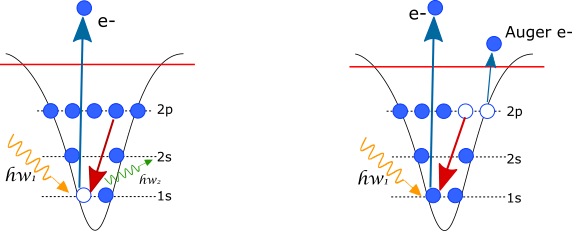
\includegraphics[width=12 cm]{../Images/text6418.png}
\caption[Relaxation processes for photoionization]{Two example on the relaxation processes. On the left, A photon ionized an electron and the Electron $E_{in}$ replaced, expelling a fluorescent photon in the process. On the right, the energy released by the replacement electron is enough to make another electron in the outer shell to also go to the continuum, Auger electron. Taken form \cite{rafipoor_two-color_2017}}
\label{fig:augerfluorec}
\end{figure} 

In example. As shown in fig \ref{fig:augerfluorec}, if a photon  with energy $\hbar\omega > E_{bin}$  ionized an electron, this will leave the atom lifting a gap. An electron in the higher levels will replace the outer one, leaving an excess of energy. The outcome will be a fluorescence process with $E_{flu} = E_{in}- E_{out}$ or , the Auger $e-$, if $ E_{in}-E_{out} > E_{bond}$ and this electron can also escape the atomic Coulomb potential \cite{schmidt_electron_1997}.



\subsection{Multiphoton and Tunnelling Ionization}

Ionization is also possible, even when the photon energy is lower than the binding potential. Laser Fields with intensities below $I \leqslant 10^{14}$ W/cm$^{2}$ are not strong enough to change the binding potential of an atom significantly \cite{rhodes_multiphoton_1985} and it is when multiphoton Ionization takes place (MPI).  MPI is the simultaneous absorption of several photons to overcome the ionization barrier. The way MPI occurs depends on the laser frequency and intensity. When the intensity is much lower than the characteristic atomic resonance, MPI occurs via transitions through virtual states. Ionization by several photons at low laser intensities can be realized by the so-called resonance enhanced multiphoton ionization (REMPI) \cite{mainfray_multiphoton_nodate}.  Ionization by a REMPI process takes place in two steps. First, a resonant excitation by one or more photons occur on an electron state of the atom. In the second step, this electron state is transformed into a virtual state, to an upper state until the electron is excited by spontaneous decay. So for example, the total energy absorbed by an election until it gets ionizes is $n * \hbar\omega > I_{pot}$ where $n$ is the number of photons absorbed until it actually have enough energy to overcome the potential $I_{pot}$

For Laser intensities $I > 10^{14}$ W/cm$^{2}$,  with higher intensities and lower frequencies, tunneling ionization (TI) is more likely to occur.  In this case, the binding potential of the atomic state is strongly affected by the electric field of the laser. Around the peak of the electric field the  potential gets narrower, and the electron in the outer states gets closer to the bidding barrier, allowing the electron to tunneling through the confining potential to the continuum  \cite{griffiths_introduction_2013}. TI is inherently a quantum process. The bending of the Coulomb potential becomes by the superposition of the coulomb potential and the laser field. Therefore TI must occur when the time of the ionization is shorter than a laser oscillation cycle\cite{berkowitz_photoabsorption_1979}. Based on the same principle, when the laser field becomes so strong to lower the binding potential that separates the highest electron level, then the electrons in this state become free electrons. This process is called barrier suppression ionization or BSI\cite{krishnan_doped_2011}.

In Fig. \ref{img:ionizationprocess}, we present a sketch of the 3 possible ionization processes explained above. On the left, a simple ionization process where a photon with energy $E_{phot} = \hbar\omega$ is higher than the potential barrier. In the center, a MPI process is shown, $n$ photons excite the inner-shell electron, exiting it through a virtual level until it finally has enough energy to be free to the continuum. Finally on the left, a TI happens. Here the coulomb potential barrier is affected by the laser files bending, the outer shell electron gets closets to it until it tunnels \cite{rafipoor_two-color_2017}.

\begin{figure}[h!]

\centering
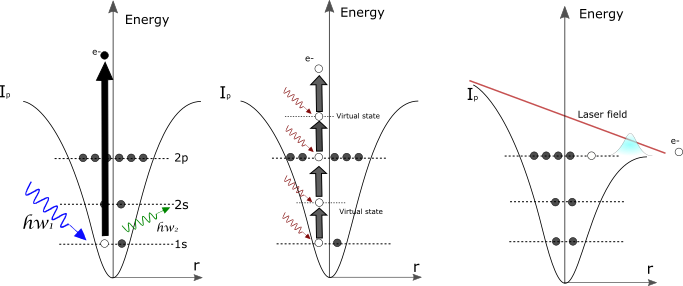
\includegraphics[width = 14 cm]{../Images/photoionization2.png}
\caption[Ionization regimes]{ On the left is the sketch of a single photon ionization process, where a photon with energy $E_{phot} = \hbar\omega$ is higher than the potential barrier $I_{p}$. On the center the MPI process, inner-shell electron absorbs $n$ photons, getting excited through the electronic levels (reals or virtual) until it reaches the continuum. On the left the BSI Process, the coulomb potential barrier bends by the laser fields, been lower than the outer shell electron state, the electrons can scape easilly. Based on \cite{rafipoor_two-color_2017}.}
\label{img:ionizationprocess}
\end{figure}


As explained the Intensity of the external field plays an important role in the ionization process. A rather easy way to differentiate when each process needs to be taken into account is provided by the Keldysh parameter\cite{keldysh_ionization_1965}.

\begin{equation}
\gamma_{k}=\sqrt{\dfrac{I_{p}}{2U_{p}}}
\end{equation}

Where $\gamma_{k}$ is the Keldish parameter, $I_{p}$ is the atoms ionization potential and $U_{p}$ is the ponderomotive potential defined as:

\begin{equation}
U_{p} = \dfrac{e^{2}E_{0}^{2}}{4m_{e}\omega_{0}^{2}} \propto I \lambda^{2}
\end{equation}

Where $m_{e}$ is the mass of the electron, $\omega_{0}, \lambda, I$ and $E_{0}$ are the frequency, wavelength, intensity and the peak of the electric field of the laser pulse. On one hand, when the Keldish parameter is higher, $\gamma_{k} \gg 1$ MPI regime is considered. On the other hand, the $\gamma_{k} \ll 1$ describes the TI interaction.

\subsubsection{ Keldysh Theory}

In this section we will give a brief introduction to the keldysh theory based on the work of Keldy et al, \cite{keldysh_ionization_1965}, and the papers review of the theory by \cite{popruzhenko_keldysh_2014} and \cite{karnakov_strong_2009}. For a deeply explanation we recommend the reader to reference this works.

The keldysh Theory, also known as the Keldysh–Faisal–Reiss theory (KFR), is well used for the description of quantum process induced by intense laser radiation. The applications and advantages of Keldysh formulation in many-body theory among  several, can overcome from, treatment of systems away from thermal equilibrium, solutions in  super symmetry methods of systems with quenched disorder or to the  calculation of the full counting statistics of a quantum observable \cite{kamenev_introduction_nodate}.

According to the Keldysh Ansatz, the transition probability amplitude between an atomic bound state and the continuum by the value of the photoelectron momentum $p$ measured at the detector is given by \cite{popruzhenko_keldysh_2014}.
 \begin{equation}
 M_{k}(p) = -\dfrac{i}{\hbar} \int_{\inf}^{+\inf} \langle \Phi_{p}\mid  V_{int}(t)\mid \Phi_{0} \rangle dt
 \end{equation}

Where $M_{k}$ denotes the Keldysh transition probability, $\Phi_{0}$ is the bond state wave function unperturbed and $\Phi_{p}$ is the canonical momentum, equal to $p$, also known as the Volkov function, and $V_{int}$ is the electron field interaction operator. If the amplitude of ionization $M_{k}(p)$ is known, the differential probability to find the photoelectron in the elementary volume near the momentum $p$ is given by the momentum distribution of the photoelectrons 

\begin{equation}
dW(p)=\mid M(p)\mid^{2} d^{3}p
\end{equation}
 Giving a total probability of
 \begin{equation}
 W= \int \mid M(p)\mid^{2} d^{e}p
 \end{equation}
 
Meaning that, for enough long pulses, containing a large number of optical periods so that its electromagnetic field is close to a periodical function of time close to the initial, it is physically more appropriate to use probabilities per time unit (rates) instead of time-integrated values.

\subsubsection{Ponderomative Energy}


As soon as an electron is released into the continuum, it starts to be under the influence of the external laser field. A description of the energy that it acquires during this interaction is given by the ponderomotive energy (PE).

\begin{equation}
U_{p} = \dfrac{e_{2}E_{a}^{2}}{4m \omega^{2}}
\end{equation}

Where $m$ and $e$ is the electron mass and charge, $E_{a}$ and $\omega_{0}$  amplitude and frequency of the electric field respectively. The formula of the ponderomotive force can be easily derived as shown in \cite{protopapas_atomic_1997}\cite{connerade_highly_1998}. Let`s consider a polarized electric field (in a.u).

\begin{equation}
E=\widehat{z}E_{a}sin(\omega_{0} t) 
\end{equation}

Considering only the $\widehat{z}$-components so we can avoid the vector sign. By classical mechanics we have.

\begin{equation}
p(t)=-\int_{t_{0}}^{t} E(t\prime)dt\prime = \dfrac{E_{0}}{\omega} (cos(\omega_{0} t)- cos(\omega_{0} t_{0}))
\end{equation}

The term on the left of the parenthesis is known as the time varying Quiver terms, and on the one on the right, reefers to the drift motion. 
Expressing the fields in terms of vector potential we will have

\begin{equation}
E(t) = \dfrac{\delta A(t)}{\delta t}
\end{equation}

\begin{equation}
p(\infty) = A(t_{0}) = -\int_{-\infty}^{t} E(t) dt = \dfrac{E_{0}}{w} cos(w_{0}t_{0})
\label{eq:pmax}
\end{equation}

in the case where the pulse  duration is big $t \longrightarrow \infty$ the $p + A(t) = 0$. This means that the momentum acquired by the electron will depend on the phase it is realized $wt$. Since the electron can be unbound in any phase of the laser pulse, will have an average kinetic energy described by

\begin{equation} 
U_{p} = \dfrac{1}{2\pi} \int (-\dfrac{E}{w} cos (wt))^{2}d(wt) = \dfrac{E^{2}_{0}}{4w^{2}_{0}} = \dfrac{p_{max}}{2}^{2}
\label{eq:pondeenergy}
\end{equation}

The pondemorotive energy also gives the maximum momentum that an electron can acquire (eq. \ref{eq:pmax}), given at the maxima. The $\omega t$ phase relation, defines what it called\textit{the three step model} showed in figure \ref{fig:ponder} . The first step corresponds to $\omega t < \pi /2$ where the laser field is suppressed, and as explained above, TI or BSI can take place. The second step, is where $\omega t > 3\pi /2$, on contrary step 1 the potential barrier is enhanced, electrons in the continuum that was winning kinetic energy are caught by the potential again, being driven  back to the atom. Finally the step 3 at phase $\omega t = n* \pi$, for $n 0 1,2,3...$. At $n=2$ it is called "recollision process" of the electron. Where the electron can be caught by the potential again, and the excess of energy release another bound electrons, depending on the kinetic energy necessary \cite{krishnan_ignition_2012}

\begin{figure}[h!]\label{fig:ponder}
\centering
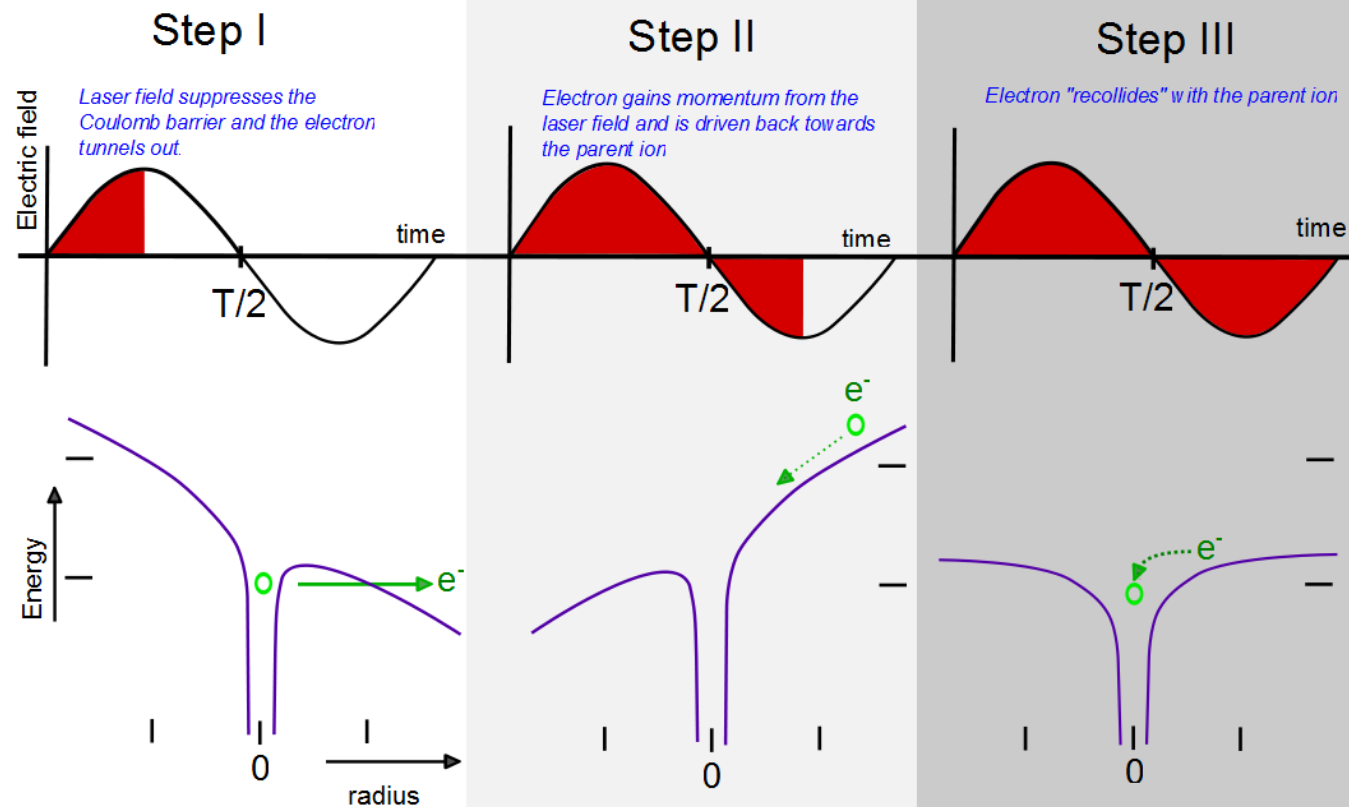
\includegraphics[width=12 cm]{../Images/ponderomotive steps.png}
\caption[Ponderomotive 3 steps]{Recollision  process at the three step model. Taken from \cite{krishnan_doped_2011}}
\label{fig:ponder}
\end{figure}


If we transform the eq. \ref{eq:pondeenergy} to laser intensities we will have $U_{p} = 9,33*10^{-14} I[W*cm^{-2}] \lambda^{2}[\mu m]$. For a MIR-pulse with intensities $\sim 10^{14}$ W/cm$^{2}$ and $\lambda \sim 3200$ nm we have electron energies between one and a hundred of eV.

\subsection{Cluster Ionization}

Until now, we have described the most known ionization processes for single atom. But on cluster ionization, the dynamics are more complex and involve more parameters. Clusters are combinations of atoms or molecules which, depending on their species, are held together by Van der Waals forces, ionic bonds or metallic bonds. In this explanation we refer from now on only to He cluster, which mainly are just affected by Van der Waals attraction\cite{stienkemeier_spectroscopy_2006} and its interaction with the Laser Fields, specifically pulsed laser with  a wavelength smaller than the cluster size, meaning that all the atoms in the cluster are equally affected by the pulse, in other words the Field penetrates all over the cluster.

The first challenge to overcome when working with Helium, is its Ip. Being a rare gas, its ionization potential is higher than many of its doping molecules used. For example, under MIR lasers helium clusters need $I > 10^{15}$ W/cm$^{2}$ , so TI or BSi is not the main process at the beginning of the plasma generation. Other interactions have to be explained in order to describe the process properly. This section we will be based on \textit{Saalaman et. al} work \cite{saalmann_mechanisms_2006} and \textit{Grüner et. al} \cite{gruner_femtosekundenspektroskopie_2013}, for this purpose, we will divide the process in three phases or stages.


In the first stage called \textit{“atomic ionization”}, the doping atoms are ionized independently of each other by the electric field at the leading edge of the laser pulse, it occurs mainly through inner ionization, especially on TI or BSI. The resulting free electrons acquire positive kinetic energy and have two options, leaving the cluster or they stay inside the cluster attracted to its positive ion core. After the first stage, the cluster becomes into an "ignited” nanoplasma, consisting of ions and quasi-free electrons, electrons that are free to travel inside the cluster volume but still not into the continuum \cite{last_quasiresonance_1999}. 


The second stage is the  \textit{nanoplasma expansion}. During this stage the cluster is still interacting with the laser field, acquiring, by a large number of processes, energy by its atoms and electrons. Ions are further created by a combined force of the laser and other ions, the \textit{ionization ignition}\cite{gruner_femtosekundenspektroskopie_2013}. Quasi-free electrons oscillate, driven by the laser pulse and are heated to high temperatures. The heating becomes extremely efficient when the collective oscillations of quasi-free electrons become resonant with the laser pulse, Triggering a cascade reaction to more outer ionizations,  freeing the remaining electrons in the cluster, this process is called \textit{plasma resonance}\cite{saalmann_mechanisms_2006}.


After the laser pulse is over, the last stage starts. The ions continue to expand, in consequence, the radius rises as same as the cluster potential becomes smoother. So, it is easier for the highly energetic quasi-free electrons to leave the cluster, forming a coulomb explosion that destroys the cluster in a ions-electrons cascade. This process was first described by \textit{Ditmire et. al} \cite{ditmire_interaction_1996} combining high energetic collisions with cluster resonance absorption.

The graphic \ref{img:clusterpotential} shows on the left how the cluster potential is composed by the Van der Waals potential and atomic forces of the different atoms that compose the cluster. On the central images, additional to the atomic biddings, the electrical force due the ions in the cluster increase the potential, the laser pulse is still on and the quasi-free electron will gain energy while they are in this. Finally, on the right the laser field is off, the electrons have fled away and the cluster ion have been repelling each other so the potential is reduced to the minimum(just atomic interactions.)

\begin{figure}[h!] \label{img:clusterpotential}

\centering
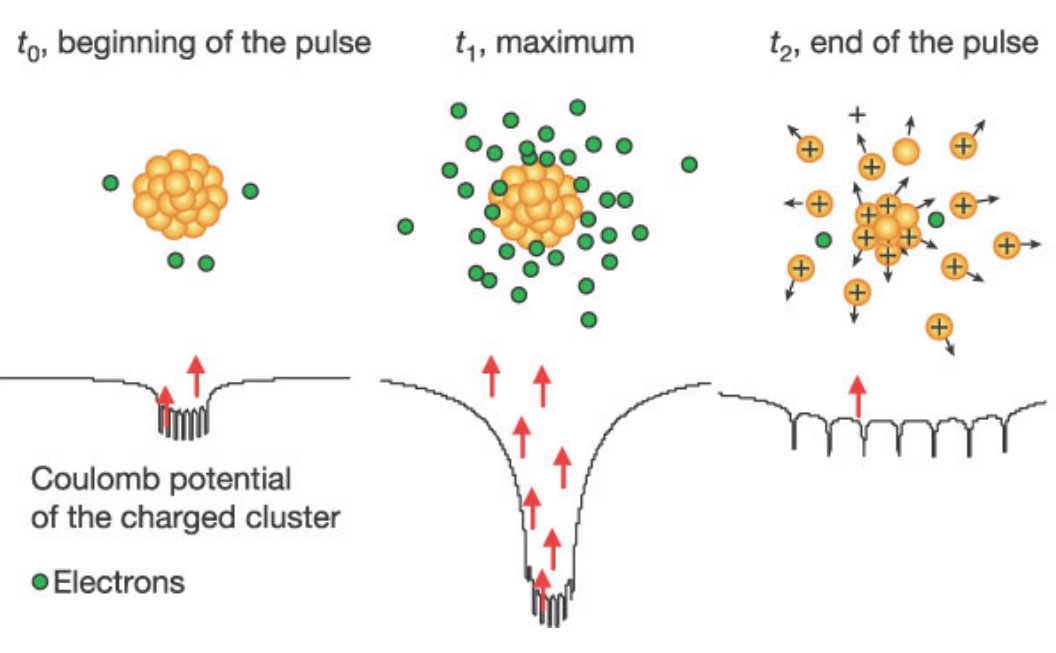
\includegraphics[scale=0.35]{../Images/clusterpotential.PNG}
\caption[Cluster potential regimes]{Cluster potential regimes. On the left, the atomic ionization starts the plasma formation. On the center, the quasi-free electrons auto-ionize the cluster, increasing the potential barrier and gaining energy due the laser field so a coulomb explosion can take place. On the right, The Coulomb explosion is finished, the potential is driven to it minimum and all the electrons and ions are ejected. Taken from \cite{wabnitz_multiple_2002}}.
\label{img:clusterpotential}
\end{figure}

Depending on the droplet size and the laser intensity, the Cluster can expand in two different ways. If the laser intensity is rather high and the droplet is small, a Coulomb explosion can occur. On the contrary, if the laser is not intense enough or the droplet is too big, a nanoplasma can be generated, therefore a hydrodynamic expansion will take place. 
Two forces are really important during the cluster expansion. Both act on the cluster during the phase two and three (during and after the laser pulse). The first, is the force associated with the free electrons with high kinetic energy. These hot electrons expand and pull the low energetic electrons and heavy ions on its pad \cite{ditmire_interaction_1996}. The other force acting on the cluster is due to the inner cluster charge itself. The hottest electrons in the cluster will have a mean free path large enough so they can free stream directly out of the cluster, and, if the electron’s energy is large enough to overcome the space-charge buildup on the cluster, they will leave the cluster altogether. If the charge buildup is sufficiently large, the cluster will undergo a Coulomb explosion \cite{haught_formation_1970}. According to Madison et all, a time scale for the laser pulse duration where the coulomb explosion can take place should be closer or lower to the femtosecond regime, depending on the element composing the cluster. \cite{madison_role_2004}. Based on the laser power available on modern laser pulses, the same studies present that electron after a coulomb explosion can get kinetic energy up to 6KeV.


When the intensity is not enough to make the atomic bonds to break, the electrons remain in the cluster forming a hydrodynamic expansion as a result of a conversion of electron-thermal energy to direct kinetic energy \cite{erk_nobel_2009}. The effects that the expansion has on the electron temperature can be calculated by equating the rate of change of radial kinetic energy from the thermal contribution with the rate of change of thermal energy within the cluster. When this condition is fulfilled. The electron can present a resonance condition in the cluster, traveling in the space-charged forces formed by the plasma, winning enough kinetic energy until all the system collapse.

\begin{figure}[h!]
\centering
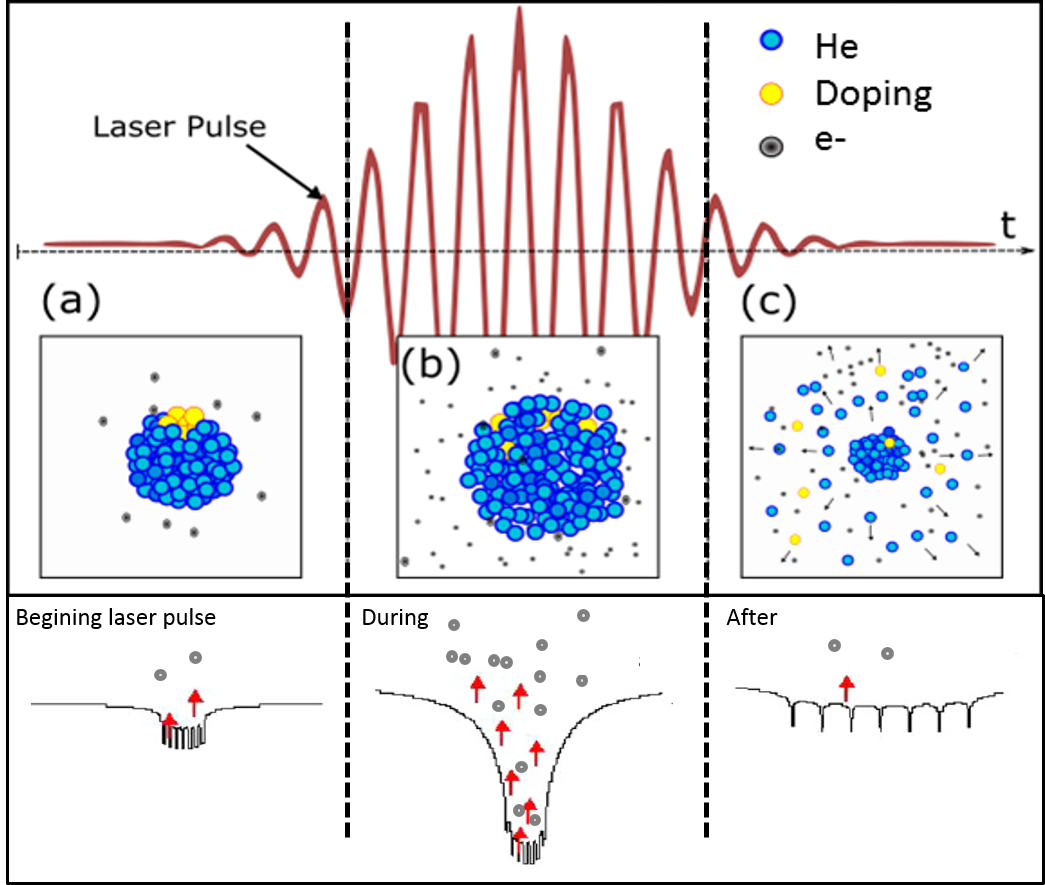
\includegraphics[width=14cm]{../Images/cluster_regimes_2.png}
\caption{sketch of the Coulomb explosion for a doped cluster due the excitation of a pulsed laser field. At the beginning of the process the laser ionized the droplet, until some femtoseconds (up to 500fs) after, the system collapse and result into a coulomb explosion.}
\label{fig:columbexplosion}

\end{figure}


Although the two models are different in each regime, for example, at low kinetic energy or the beginning of the pulse, the Coulomb explosion produces less ions for low energies compared to the product on hydrodynamic explosions. Further, the number of high energy ion the coulomb explosion can create (although in less quantity) tent to be hotter ions too.
We have to take into account that even the two processes are described for different laser regimes. Both processes can happen in parallel, but at certain energies is clear, that one or the other will be the responsible at the end, for the collapse of the system.

\subsection{Homogeneous Charge Sphere  Model}

Once the ionization process started, an electronic cloud of quazifree electrons will be created around the remaining cluster. This is a complex physical process due its chaotic system determined by the individual velocity vectors of the particles and their interaction between the Electric field, the cluster and each other. Various theoretical approaches ranging from phenomenological models \cite{ditmire_interaction_1996} to large-scale microscopic calculations \cite{saalmann_mechanisms_2006} have been done but far for been interpreted to clusters and system with more than a few thousand of particles. Additional a  theoretical scenario of a single well-characterized cluster, irradiated by a laser pulse of a given intensity is usually far from the real experimental situation. An analytical solution is far from been formulated, we work joint to the theoretician Andreas Heidenreich to make computational simulations. This are demanding simulations that takes a large of computational power even for small cluster, the results can recreated reasonably the experimental system and so give a better background to the understanding of the plasma formation.

Another, more simple and intuitive approach is done by  \textit{Ranaul Islam et al.}, in \cite{islam_kinetic_2006} they try to express the kinetic energy distribution for an ion cloud. Two important assumptions are made for this model. First, we assume a uniformly charge distributed spherical cloud with radius $R$ and density $\rho=N/vol$ where $N$ is the number of particles inside the sphere, furthermore all the particle lays with zero kinetic energy. Second, The basic mechanism underlying the kinetic energy distribution in clusters is their Coulomb explosion, it converts the potential energy $E_{coul}$ of a partially ionized cluster atom at a distance $r$ from the cluster center into kinetic energy $E$. The probability $dP/dr$ to find an atom at a distance $4$ from the cluster center is then given by\cite{islam_kinetic_2006}

\begin{align}
\frac{dP}{dr}=\frac{3 r^2}{R^3} \Theta (R-r)
\label{density_distribution}
\end{align}

where, $\frac{dP}{dr}$ is the probability to find an electron at radius $r$ and $\Theta$ is the step function for the particles inside the radius of the sphere, with homogeneous charged density, we have $N$ particles with a charge of $q$ and just after the are ionizes they have not moved yet, then the potential Coulomb energy of an particle inside the cluster is given by

\begin{align}
E_{coul}(r)=Ne^2 \frac{r^2}{R^3}
\label{coulomb_energy}
\end{align}

for $r\leq R$. $N$ is the number of electrons in the sphere and $e$ is the elementary charge of an electron. A charged sphere like this will immediately coulomb explode and for $t \longrightarrow \infty$ all coulomb energy is converted to kinetic energy, which can be measured experimentally with the VMI. It is possible to retrieve the energy distribution out of the spatial distribution \ref{density_distribution} with \ref{coulomb_energy} as the substitution formula.

\begin{align}
dr=\frac{R^3}{2Nq^2r}dE
\label{substitution}
\end{align}

Furthermore, we define the maximum coulomb energy

\begin{align}
E(R):=E_R=Nq^2 \frac{1}{R}
\label{max_coul_energy}
\end{align}

with all this follows the energy distribution of the electrons

\begin{align}
\frac{dP}{dE}=\frac{3}{2} \sqrt{\frac{1}{E_R}} \frac{1}{E_R}\sqrt{E} \cdot \Theta (1-\frac{E}{E_R})
\end{align}

it can be seen, that the energy distribution is fully characterized by $E_R$, so it is enough to know the maximum kinetic energy, which is just the radius of the central feature in our VMI images. With this even the inverse Abel transformation can be bypassed, because the edge of a sphere in invariant for projecting the sphere on a plane.
\begin{figure}[hbtp]

\centering
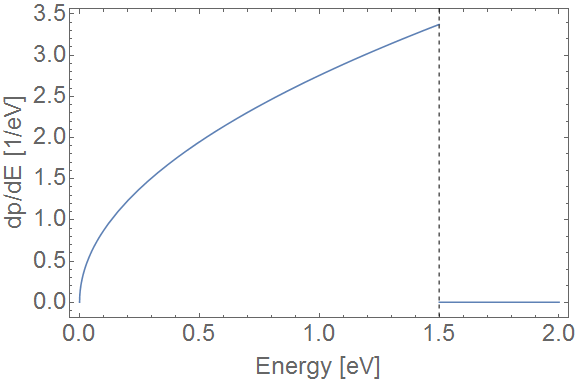
\includegraphics[scale=0.4]{../Images/linemodelfit.png}
\caption[Islam Model fit]{Energy distribution for a coulomb explosion of a full sphere of electrons according to formula 3.10. The dashed line marks cutoff energy E$_{R} $}
\end{figure}


With the formula for the homogeneous density in a sphere

\begin{align}
R=(\frac{N}{\frac{4}{3} \pi \rho})^{1/3}
\end{align}

and formula \ref{max_coul_energy} the charge density in the beginning in the process can be derived to

\begin{align}
E_{max}(N)=\underbrace{\frac{e^2}{4 \pi \epsilon_0} (\frac{4}{3} \pi \rho)^{1/3}}_{=:B} N^{2/3}
\end{align}

and with this the charge density reads

\begin{align}
\rho=48 \pi^2 \frac{\epsilon_0^3}{e^6} B^3
\end{align}

In summary, the charge density can be calculated with the fit parameter $B$ or B-factor as we will named from now on.  $B$ can be retrieved by plotting the maximum kinetic energy $E_R$ as a function of the number of electrons $N$. Both can be extracted out of the VMI images, $E_R$ from the radius and $N$ from the brightness of the central feature.

